\input{../common}

\begin{document}
  %<*content>
  \lesson{analysis}{27}{Dénombrement}
  
  
  ${\color{blue}\blacktriangleright } $  Combien peut-on attribuer de numéros de téléphones portables (numéros à 9 chiffres commençant par 77)?\\

 ${\color{blue}\blacktriangleright } $ Huit athlètes prennent le départ d'une course. Combien y a-t-il d'arrivées possibles? \\

$ {\color{blue}\blacktriangleright } $ Combien y a-t-il de façons de sélectionner une équipe de 11 joueurs parmi les 22 membres d'un club? \\

Ces questions constituent des exemples simples de problèmes de  dénombrement. \\
L'objet de ce chapitre est de mettre en place des outils pour les résoudre. \\
 Signalons que le dénombrement est particulièrement utile en probabilité. 


\subsection{Ensemble fini - Cardinal}
\begin{definition}
Soit $ n$ un entier naturel.\\
Lorsqu'un ensemble $ E $ a $ n $ éléments, on dit que $ E $ est un ensemble  fini de cardinal  $ n. $  \\
On note alors  card$ E $ = $n$. 
\end{definition}
\begin{example}
\begin{enumerate}
\item  $ E= \accol {a, b, c}$ est un ensemble fini et card$ E $ = $3.$
\item Si $ E =\varnothing $, il comporte zéro élément et  card$ \varnothing =0$
\item Certains ensembles ne sont pas finis tels que $ \Nn $, $ \Rr $, $ \intff{0}{1} $
\end{enumerate}
\end{example}
\begin{remark}

Résoudre un problème de dénombrement consiste généralement à déterminer le cardinal d'un ensemble fini E. Le problème se pose en général lorsque E est donné en compréhension, c'est-à-dire par une description de  ses éléments.  \\  L'objet de ce qui suit est de trouver des méthodes simples pour calculer des cardinaux d'ensembles finis.
\end{remark} 
\subsection*{Partie d'une ensemble}
\begin{definition}
Soient $A $ et $ E$ deux ensembles finis.

 $ A $ est une partie ou  un sous-ensemble de $ E $ si tout élément de $ A $ est élément de $ E. $  On note $ A \subset E $ (lire $ A$ inclus dans $E $).

\end{definition}
\subsection*{Intersection et réunion}
Soient $A $ et $ B $ deux parties d'un ensemble   $E. $
\begin{definition}
\begin{itemize}
\item[\textbullet] L'ensemble des éléments communs à  $A $ et $ B $ est appelé intersection de $A $ et $ B$; noté $ A\cap B $  (lire A inter B).

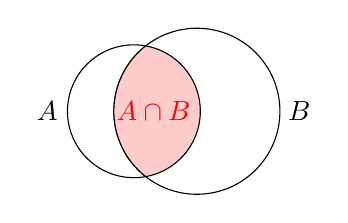
\begin{tikzpicture}[scale=1]

	\draw (0.8,0) circle (30pt);
	
	\begin{scope}
	\clip (0,0) circle (24pt);
	\fill[fill=red!20,draw=black] (0.8,0) circle (30pt);
	\end{scope}
	
	\draw (0,0) circle (24pt);
	\node at (-1.1,0) {$A$};
	\node at (2.1,0) {$B$};
	\node[red] at (0.25,0) {$A\cap B$};

\end{tikzpicture}
\item[\textbullet] L'ensemble des éléments qui appartiennent  à  $A $ ou à $ B $ est appelé réunion de $A $ et $ B$; noté $ A\cup  B $  (lire A union B).

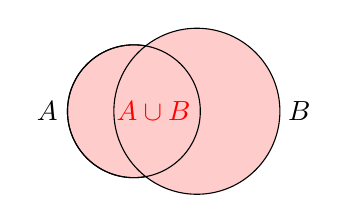
\begin{tikzpicture}[scale=1]

	\fill[fill=red!20,draw=black] (0,0) circle (24pt);
	\fill[fill=red!20,draw=black] (0.8,0) circle (30pt);
	\draw (0,0) circle (24pt);
	\node at (-1.1,0) {$A$};
	\node at (2.1,0) {$B$};
	\node[red] at (0.25,0) {$A\cup B$};

\end{tikzpicture}
\end{itemize}
\end{definition}
\begin{example}
Considérons les ensembles  suivants:  $ A=\accol{5;0;1;6}$  $ B=\accol{1;6;7} $.

On a $A\cap B = \accol{1; 6} $, $A\cup B = \accol{0;5;1;6;7}$.

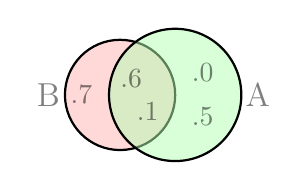
\begin{tikzpicture}[thick,fill opacity=0.5, scale=0.7]
\filldraw[fill=red!30] (0:1cm) circle (10mm);
\filldraw[fill=green!30] (0:2cm) circle (12mm);
\node at (-0.3,0) {\large B};
\node at (3.5,0) {\large A};
\node at (1.5,-0.3) { .1};
\node at (1.2,0.3) { .6};
\node at (0.3,0) { .7};
\node at (2.5,-0.4) { .5};
\node at (2.5,0.4) { .0};
\end{tikzpicture}

 \end{example}
\begin{remark}

$ \centerdot $ $A\cup B$ est l'ensemble des éléments qui appartiennent  au \textbf{moins} à A ou B.\\
$ \centerdot $ Lorsque $ A$ et  $ B$ n'ont aucun élément en commun, on dit qu'ils sont \textbf{disjoints}; donc on a: $ A\cap B=\varnothing $ Dans ce cas  $A\cup B$  est l'ensemble des éléments qui appartiennent à A \textbf{ ou bien} à B.
\end{remark}
\begin{property}
                 \[\textrm{card}(A\cup B)= \textrm{card}A  + \textrm{card}B- \textrm{card}(A\cap B)    \]
                  \[ \textrm{Si}\  A\cap B=\varnothing \quad \textrm{alors}\quad \textrm{card}(A\cup B)= \textrm{card}A  + \textrm{card}B    \]
\end{property}
\begin{exercice}

Dans une classe de 30 élèves, 19 élèves font espagnol, 18 élèves font arabe comme deuxième langue facultative. Sachant que tous les élèves étudient au moins l'une des deux  langues. Détermine le nombre d'élèves qui étudient les deux langues à la fois.
\end{exercice}


\begin{proof}

Soit $ A $ l'ensemble des élèves qui étudient l'espagnol et $ B $ celui de ceux qui font arabe donc l'ensemble des élèves qui étudient les deux langues à la fois est $A\cap B.  $ Soit $ x $ son cardinal. \\
$ A\cup B $  est l'ensemble des élèves de la classe d'effectif $ \textrm{card}(A\cup B)=30 $\\
$ \textrm{card}(A\cup B)= \textrm{card}A  + \textrm{card}B- \textrm{card}(A\cap B)    $\\
$\textrm{card}(A\cup B)= 19+18-x=30  $\\
 On trouve $ x=7 $ c'est à dire 7 élèves étudient les deux langues à la fois.
 \end{proof}
\begin{remark}
Pour le cas de trois ensembles, il est conseillé de s'aider de diagrammes.
\end{remark}

\subsection*{Complémentaire}
Soit  $ A $ une partie d'un ensemble  $ E $
\begin{definition}
 Le  complémentaire de $ A $ dans $ E $,  noté $ \overline{A} $, est l'ensemble des éléments  de $ E $ qui ne sont pas dans $ A. $
 
 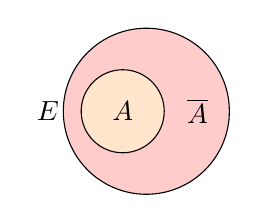
\begin{tikzpicture}[scale=1]

	\fill[fill=red!20,draw=black] (0.3,0) circle (30pt);
	\fill[fill=orange!20,draw=black] (0,0) circle (15pt);
	\node at (0,0) {$A$};
	\node at (0.95,0) {$\overline{A}$};
	\node at (-0.95,0) {$E$};

\end{tikzpicture}
 \end{definition}
\begin{example}
$ E=\accol{0;1;2; \cdots ; 2017} $\\
Si $ A=\accol{0;1;2;3; 4} $ alors  $ \overline{A}=\accol{5;6;\cdots ;2017} $ 
\end{example}


\begin{property}[Cardinal du complémentaire]
\[ \textrm{card} \overline{A} = \textrm{card}E - \textrm{card}A  \]
\end{property}
 Parfois, il sera plus simple dans un exercice où l'on a les locutions << au moins >> ou << au plus>>, de dénombrer le complémentaire de  A dans un ensemble   E connu et d'utiliser l'égalité précédente.

\subsection*{Produit cartésien}
\begin{definition}[Cas de deux ensembles]
Soient $A $ et  $B $ deux ensembles finis non vides.\\
On appelle  produit cartésien de $ A$ par $B $, noté $A\times B$  (lire $ A $ croix $ B $), l'ensemble des couples $ \paren{x, y} $ où $x\in A $ et $y\in B. $
\end{definition}
\begin{example}

Prenons $ A=\accol{a, b} $ et $ B= \accol{1; 2; 3} $\\
On a alors $ A\times B=\accol{(a, 1); (a, 2);(a,3);(b,1);(b,2);(b,3)  } $
\end{example}
\textbf{Cardinal du produit cartésien}\\
Considérons toujours  les deux ensembles :\;$ A=\accol{a, b} $ et $ B= \accol{1; 2; 3} $\\
On a $ A\times B=\accol{(a, 1); (a, 2);(a,3);(b,1);(b,2);(b,3)  } $\\
Un élément de $ A $ est dans $ 3 $ couples alors les $ 2 $ éléments de $ A $ seront dans $ 2\times 3 $ couples.\\  Donc card$( A \times B) = 2\times 3 =6$\\ D'une manière générale:

\begin{theorem}

\[ \textrm{card}( A\times B) = \textrm{card}A \centerdot \textrm{card}B  \]

\end{theorem}


\begin{remark}

Lorsque $ A\neq B $ on a $ A \times B \neq B \times A $ car un couple est ordonné \\Par contre card $( A\times B )=$ card $ (B\times A) $ quels que soient $A $ et $B $
 \begin{itemize}
 \item[\textbullet]  Cette définition s'étend à un nombre quelconque d'ensembles finis:  le produit cartésien de trois ensembles finis A, B et C est  l'ensemble noté A$\times$B$ \times$C  et card( A$\times$B$ \times$C) =cardA.cardB.cardC.
 \item[\textbullet] Les éléments du  produit cartésien  de deux ensembles sont appelés couples; les éléments du  produit cartésien  de trois ensembles sont appelés triplets; les éléments du  produit cartésien de $ p $ ensembles  sont appelés p-uplets \; ( $ p\geq4) $.
  \end{itemize}
 
 \end{remark}
 
 \begin{corollary}[Le principe multiplicatif] 
Pour dénombrer un ensemble, on peut utiliser le principe suivant:\\
Si une situation comporte $ p $  étapes successives offrant chacune $ n_{i} $ possibilités (ou choix) alors le nombre total de possibilités d'effectuer cette situation dans l'ordre indiqué des étapes est :
$   n_{1}\times n_{2} \times \cdots \times n_{p} $
\end{corollary} 

 
 
 \begin{example}

Le  menu d'un restaurant propose un certain jour pour le repas de midi 3 entrées, 4 plats de résistance et 2 desserts. De combien de façons un client peut-il composer son menu ce jour-là ? 

    Le choix d'un menu est une situation qui comporte 3 étapes :\\
 choix d'une entrée : 3 possibilités\\
choix d'un plat de résistance  : 4 possibilités\\
choix d'un dessert : 2 possibilités.\\
D'après le principe multiplicatif, le nombre total de choix possibles est :  $ 3 \times 4 \times 2 = 24$  menus.
 \end{example}
 
 \begin{exercice}
Un homme, pour se rendre à un mariage doit choisir la veste,  la chemise  et un pantalon. Sachant qu'il dispose de 2 vestes, 4 pantalons et 3 chemises, de combien de façons peut-il effectuer son choix? 
   \end{exercice}
 
\textbf{A retenir}\\
 Dans une situation de dénombrement, lorsque les différentes étapes sont liées par la conjonction de coordination  << et>>   alors il faut faire une multiplication.

\subsection*{Partition d'un ensemble}
\begin{definition}
Soient $ B_{1}, \; B_{2}, \cdots, B_{p} $ des  parties non vides d'un ensemble fini $ E. $  On dit qu'elles forment une partition de $ E $ si:
\begin{itemize}
\item[$  \bullet$] elles sont deux à deux disjointes 
\item[$  \bullet$]  et  $B_{1}\cup B_{2}\cup  \cdots\cup B_{p} =E $\; (\textit{leur réunion donne E})
\end{itemize}
\end{definition}

\bigskip
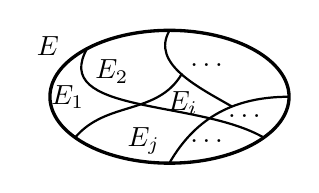
\begin{tikzpicture}[scale=0.8]

	\draw[very thick] (0,0) ellipse (54pt and 30pt);
%	\fill[myred] (0,0) circle (2pt);

	\path[-, thick] (0,-1.05) edge[out=60,in=180] (1.9,0);
	\path[-, thick] (0,1.05) edge[out=-120,in=150] (1,-0.16);
	\path[-, thick] (0.2,0.37) edge[out=-120,in=50] (-1.5,-0.65);
	\path[-, thick] (-1.3,0.78) edge[out=-120,in=150] (1.5,-0.65);

   \node[left] at (-0.5,0.4) {$E_2$}; 
   \node[left] at (1,0.5) {$\ldots$}; 
   \node[left] at (1,-0.7) {$\ldots$}; 
   \node[left] at (0,-0.7) {$E_j$}; 
   \node[left] at (-1.2,0) {$E_1$}; 
   \node[left] at (0.6,-0.1) {$E_i$}; 
   \node[left] at (1.6,-0.3) {$\ldots$}; 


   \node[left] at (-1.6,0.8) {$E$}; 
\end{tikzpicture}

\begin{example}

Soit $ E $ l'ensemble tel que $ E= \accol{a, b, c, d, e, f} $
\begin{itemize}
\item[\textbullet] les ensembles  $ \accol{a}; \accol{b, c,  f}; \accol{d,e} $ forment une partition de $ E. $
\item[\textbullet] les ensembles  $ \accol{a}; \accol{b, c,  f}; \accol{a, b,d,e} $ ne  forment pas une partition de $ E$ car ils ne  sont pas disjoints deux à deux.
\end{itemize}
\end{example}
\begin{property}
Soit $ E $ un ensemble fini et  $ E_{1}, \; E_{2}, \cdots, E_{p} $ des ensembles formant une partition de $ E. $ 
 $$ \text{On a:}\;\;   \textrm{card }E= \textrm{card } E_{1}+ \textrm{card }E_{2} + \textrm{card }E_{3}+ \cdots + \textrm{card } E_{p}$$
\end{property}
Cette propriété est appelée \textbf{principe  additif }(Nous l'admettons).\\
Pour résoudre un problème de dénombrement, il peut-être utile d'effectuer une partition de l'ensemble à dénombrer. Le cardinal de cet ensemble est alors la somme des cardinaux des   ensembles de la partition.

\textbf{ Autre formulation du principe additif}

Si une situation offre $ p $ choix comportant chacun $ n_{i} $ possibilités alors le nombre de choix possibles est :
$n_{1}+ n_{2}+ \cdots + n_{p} $

\begin{example}

 Pour aller en ville, une personne dispose de 3 vélos, 2 motos  et 4 bus.\\
Déterminer le nombre de possibilités de cette personne pour accéder en ville.

  La personne prend un vélo ( avec 3 possibilités) ou une moto ( avec 2 possibilités) ou un bus ( avec 4 possibilités) donc d'après le principe additif,  le nombre de possibilités est $ 3+2+4= 9$ 
\end{example}

\textbf{NB}: Lorsque le raisonnement amène \textbf{ou}   alors il faut faire une  addition.

\subsection{ Notion de   p-listes}

\begin{definition}

Soit $ E $ un ensemble à $ n $ éléments et $ p $ un entier naturel non nul.\\
Une p-liste, est une liste  de $ p $ éléments ordonnés et non nécessairement distincts choisis parmi les $ n $ éléments de $ E $.
\end{definition}


\begin{example}

$ \centerdot $ $ \paren{1,1,1}; \paren{0,0,1};\paren{0,0,0}; $ sont des 3-listes de l'ensemble $ \accol{0;1} $.\\
$ \centerdot $  $ \paren{P,P,F,F,F,P,F,P,F,F} $ est une 10-liste de l'ensemble $ \accol{P;F} $: il correspond, par exemple, à un résultat de 10 lancers consécutifs d'une pièce de monnaie (pile ou face).
\end{example}

\begin{remark}

Dans une  p-liste, on tient compte de l'ordre des éléments de la liste et un élément choisi peut être répété plusieurs fois dans la liste.
\end{remark}
\begin{theorem}

Le nombre de p-listes  d'un ensemble à $ n $ éléments est $ n^{p}. $
\end{theorem}

\textbf{Démonstration}

Il y a $ n $ choix possibles pour  le 1$^{\text{ier}} $ élément de la liste.\\
Il y a $ n $ choix possibles pour  le 2$^{\text{ieme}} $ élément de la liste.\\
Il y a $ n $ choix pour  le 3$^{\text{ieme}}$ élément de la liste.\\
.......................................................................................\\
Il y a $ n $ choix possibles pour le p$^{\text{ieme}} $ élément de la liste.\\
D'après le principe multiplicatif, on a $\underbrace{ n \times n \times n \times \cdots \times n }_{p\  fois}$  $\quad\textrm{ p-listes} $.

 \begin{example}

Une urne contient 15 boules numérotées de 1 à 15. On en tire trois successivement en remettant à chaque fois la boule tirée.  Combien y a t-il de tirages  possibles? \\

Soit E l'ensemble des 15 boules.\\
Les boules tirées sont ordonnées puisqu'on les tire l'une après l'autre ; elles ne sont pas nécessairement distinctes puisqu'on remet la boule tirée dans l'urne  après chaque tirage.\\
Donc un tirage est une  3-liste  de l'ensemble E: le nombre de tirages possibles est $ 15^{3} $
 \end{example}

\bigskip


\textbf{Méthode}

Dans toute situation où  l'on choisit successivement avec remise $ p $ éléments parmi $ n $ éléments, on applique la formule des  p-listes   pour déterminer le nombre de choix possibles.


\medskip
\textbf{NB}

Dans une p-liste, p peut-être supérieur à n.
\subsection{Arrangements}
\begin{definition}
Soit $ E $ un ensemble à $ n $ éléments et $ p $ un entier naturel non nul tel que $p\leq n  $ .\\
On appelle  arrangement  de $ p  $ éléments  de $ E,$   \textbf{toute  p-liste}  d'éléments de $ E $ \textbf{deux à deux distincts}.
\end{definition}
\begin{example}
 Les arrangements à trois éléments de l'ensemble $ \accol{a, b,c} $ sont: $\; (a,b,c),\;\;\; (a,c,b),\;\;\;(c,a,b),\;\;\; (c,b,a),\;\;\; (b,a,c),\;\;\; (b,c,a),\;\;$ 

\end{example}
Un arrangement de $ p $ éléments de $ E $, est une liste  de $ p $ éléments choisis parmi les $ n $ éléments de $ E $ ordonnés et deux à deux  distincts.\\
Donc dans un arrangement, on tient compte de l'ordre des éléments de la liste et chaque élément de la liste est  écrit une et une seule fois (pas de répétition).\\
\textbf{Nombre d'arrangements}
 \begin{example}
  Dix athlètes participent à une course. On appelle podium l'arrivée des trois premiers.\\
On se propose de déterminer le nombre  de podiums possibles, en supposant qu'il n'y a pas d'ex æquo.
\medskip

 Dans un  podium les 3 athlètes  sont << ordonnés >> et ne peuvent se << répéter>>. Chaque  podium correspond donc  à un arrangement de trois athlètes pris parmi 10 athlètes.
Donc il y a autant de podiums  que d'arrangements de trois athlètes pris parmi 10.\\
Déterminons le nombre de ces arrangements de $ 3$ athlètes pris parmi 10.\\
Il y a $ 10 $ choix possibles pour  la 1$^{\text{e}} $ place .\\
Il y a $ 9 $ choix possibles  pour la 2$^{\text{e}} $  place.\\
Il y a $ 8 $ choix possibles pour la 3$^{\text{e}} $ place.\\
D'après le principe multiplicatif, il y a $ 10 \times 9 \times 8 \times  $  arrangements de $ 3 $  éléments de l'ensemble à 10 éléments.  Soit  720 podiums.

 \end{example}

\begin{theorem}
Le nombre d'arrangements de $ p $ éléments  d'un ensemble $ E $ à $ n $ éléments,  noté  $ A_{n}^{p} $, est tel que :
\[  A_{n}^{p}= n(n-1)(n-2)\cdots (n-p+1)\]
\end{theorem}

\begin{example}
$A_{10}^{3} =10\times 9\times 8=720.  $
\end{example}

\begin{exercice}

 Une urne contient 11 boules numérotées de 1 à 11. On en tire quatre successivement sans  remettre à chaque fois la boule  tirée.  Combien y a -t-il de tirages  possibles? 
\end{exercice}
 \begin{proof}
 
  Le  mot << successivement >> suggère que l'ordre de tirage des boules est important et il n'y peut avoir de répétition car la boule tirée n'est pas remise dans l'urne. 
Chaque tirage correspond donc  à un arrangement de 4 éléments de l'ensemble des 10 boules.\\
Il y a donc $A_{11}^{4} =11\times 10\times 9 \times 8 =7920.  $
 \end{proof}
\begin{remark}
 
  $ \bullet $ Si $  p > n $, il est impossible de faire des arrangements.

$ \bullet $ Dans toute situation  où l'on effectue un choix de manière successive sans remise (élection de bureau avec postes, course et ordre d'arrivée...), on applique la formule des arrangements.
\end{remark}
 \begin{exercice}
L'association de 20 membres souhaite élire
\begin{itemize}
 \item[$  \ast$]   le président,
  \item[$  \ast$]  le secrétaire et
 \item[$  \ast$]    le trésorier
\end{itemize}
    Combien y-a-t-il de possibilités d'avoir ces trois responsables
   \end{exercice}
\subsection*{Notation factorielle}
$ \centerdot $ Pour un nombre  entier naturel $ n $ non nul, le produit $ 1\times 2\times 3\times \cdots \times (n-1)\times n  $ est appelé \textbf{factorielle n}  et est noté $n!$\\
$ \centerdot $ Par convention $ 0!=1 $
\begin{example}
$1!=1$\\
$6!=1\times 2\times 3\times 4\times 5 \times 6= 720$\\
$3!=1\times 2\times 3= 6$
\end{example}


\begin{property}
$ \centerdot $ Soit $ n$ et $p $ deux  nombres  entiers naturels  non nuls tels que : $ p< n $. On a  $$A_{n}^{p}= \dfrac{n!}{(n-p)!} $$
$ \centerdot $ Par convention $ A_{n}^{0}=1 $
\end{property}
\begin{example}

$A_{11}^{4}= \dfrac{11!}{7!}=\dfrac{11\times10\times9\times 8\times7\times6\times5\times4\times3\times2\times1}{7\times6\times5\times4\times3\times2\times1} =11\times 10\times 9 \times 8 =7920.  $
\end{example}
\subsection*{Permutations}
\begin{definition}
Soit $ E $ un ensemble à $ n $ éléments.\\
On appelle \textbf{permutation} de $ E $ un arrangement des $ n $ éléments de $ E. $
\end{definition}
Une permutation est un arrangement particulier (où $ n=p ) $; donc c'est un choix successif sans remise de $ n $ éléments  parmi les $ n $ éléments de $ E. $
\begin{property}
Le nombre de permutations d'un ensemble à $\; n \;$ éléments est $\;\; n!$.
 \end{property}
  
   On a aussi $A_{n}^{n}=n!$


 \begin{example} 

 Le nombre de façons de placer 6 personnes autour d'une table ronde  dont les places sont numérotées de 1 a 6 est égal à $ 6! $. 	Soit $ 1\times 2\times 3\times 4\times 5 \times 6= 720 $\; (\textit{c'est le nombre de façons de permuter les 6  personnes autour de la table})
 \end{example}
 
  \begin{example}

 Un parieur a sélectionné trois chevaux avec lesquels il veut composer son tiercé. De combien de façons  dispose-t-il pour les classer dans l'ordre? \\
 \textbf{Réponse:}  le nombre de façons est $ 3!= 6 $\; (\textit{c'est le nombre de façons de permuter les trois chevaux})
	 \end{example}
\subsection*{Notion d'Anagramme}
\begin{definition}
On appelle une  anagramme d'un mot (resp. d'un nombre), tout mot (resp. tout nombre) obtenu à partir de toutes les lettres (resp. tous les chiffres) de ce mot (resp. de ce nombre).
\end{definition}
\begin{example}
\begin{itemize}
\item[$  \bullet$] Les anagrammes du mot BAC sont: CAB, BCA, BAC, CBA, ABC, ACB.\\
Il y en a $ 3!=6 $\; c'est le nombre de permutations des lettres du mot BAC.\\
\item[$  \bullet$] Les anagrammes du nombre 123 sont: 123, 321, 213, 132, 231, 312.\\
Il y en a $ 3!=6 $\; c'est le nombre de permutations des chiffres du nombre 123.\\
\item[$  \bullet$] Les anagrammes du mot EVE sont: VEE, EVE, EEV .\\
Il y en a $ \dfrac{3!}{2!}=\dfrac{6}{2} =3$. La lettre E se répète  2 fois, donc on a divisé par $ 2! $ \\
\item[$  \bullet$] Les anagrammes du mot DENOMBREMENT sont au nombre de $ \dfrac{12!}{3! 2!2!} $\\ La lettre E  se répète  3 fois, les lettres  M et N se répètent  2 fois donc on divise par $3! $ $ 2! $ $2! $\\
\item[$  \bullet$] Les anagrammes du nombre 12322 sont au nombre de $ \dfrac{5!}{3!}=5 \times4 $

\end{itemize}
\end{example}
\medskip

\textbf{NB}:~ Les anagrammes nous  permettent de déterminer le nombre de positions des objets dans les tirages successifs.

\subsection{Combinaisons}
\begin{definition}
E étant un ensemble non vide à $ n $ éléments, $ p $ un nombre entier naturel tel que $ p\leq n. $\\
On appelle combinaison de $ p $ éléments de $ E $ toute \textbf{partie}  de $ E $ ayant $ p $ éléments.\\
On dit aussi combinaison de $ p $ éléments parmi $ n $ éléments.
\end{definition}
\begin{example}

Considérons l'ensemble $ E=\accol{a~, ~e ~, ~i ~, o~, ~u} $\\
Donnons toutes les combinaisons  à trois éléments   de $ E. $\\
Faisons le comptage: $ \accol{a; e; o} $,  $ \accol{a; i; o} $, $ \accol{a; u; o} $,$ \accol{e; u; o} $, $ \accol{e; u; i} $, $ \accol{i; u; o} $, $ \accol{i; u; e} $, $ \accol{u; i; a} $,  $ \accol{a; i; e} $, $ \accol{a; u; e} $.\\
Il y a 10 combinaisons de 3 éléments pris parmi 6 éléments.  On note par ~$ C_{5}^{3} $ ~ ce nombre  c'est-à-dire $ C_{5}^{3}=10 $.
\end{example}
\begin{remark}

Dans une combinaison, on ne tient pas compte de l'ordre des éléments et il n'y a pas possibilité  de répétition des éléments.
\end{remark}
\textbf{Nombre de combinaisons}

On note par $ C_{n}^{p} $ le nombre de toutes les combinaisons à $ p $ éléments d'ensemble à $ n $  éléments. \\Donnons des exemples de  calcul  de $ C_{n}^{p} $.\\
Exemples\;  $ C_{5}^{3}= \dfrac{  5\times 4\times 3}{ 3\times 2\times 1}=10 \;$ et $ \;C_{8}^{5}= \dfrac{8 \times7 \times6\times 5\times 4}{5 \times4\times 3\times 2\times 1}=56 $

\bigskip


On utilise aussi la formule suivante que nous admettons.
\[  C_{n}^{p}=\dfrac{n!}{p!(n-p)!} \]



$ C_{8}^{5}=\dfrac{8!}{5!(8-5)!}=\dfrac{8!}{5!3!}=\dfrac{8\times7\times6\times5\times4\times3\times2\times1}{5\times4\times3\times2\times1\times3\times2\times1}=56 $

\begin{exercice}

On tire simultanément deux jetons dans un sac contenant sept jetons numérotés.\\ Combien y a -t-il de tirages possibles?
\end{exercice}

\begin{proof}

Les jetons étant tirés en même temps (en vrac!) donc il n'y a ni ordre ni répétition des    2 jetons tirés.
Un tirage  peut être donc  modélisé par une combinaison de 2 éléments dans un ensemble contenant 7 éléments. 
Donc il y a $ C_{7}^{2} $ tirages possibles.\\

Calculons\quad $ C_{7}^{2}= \dfrac{7!}{2!(7-2)!}=\dfrac{7!}{2!5!}=\dfrac{7\times6\times5\times4\times3\times2\times1}{2\times 5\times4\times3\times2\times1} = 21$ \\

Autre façon \quad $ C_{7}^{2}=\dfrac{7\times6}{2\times1}=21 $
\end{proof}

\begin{remark}

Dans une situation où l'on effectue un choix sans ordre ni répétition (cas d'un tirage simultané), on utilise  la formule des combinaisons.
\end{remark}
\begin{exercice} 
On constitue un groupe de 5 personnes choisies parmi 12 femmes et 10 hommes
\begin{enumerate}
\item De combien de façons peut-on constituer ce groupe de 5 personnes ?
 \item De combien de façons peut-on constituer ce groupe avec  uniquement des hommes ?
\item De combien de façons peut-on constituer ce groupe avec des personnes de même sexe?
\end{enumerate}
  \end{exercice} 
   
  \subsection{Quelques exercices classiques}

\begin{exercice}

 Une urne contient 3 boules bleues, 4 boules rouges et 2 boules vertes. Les boules sont supposées indiscernables au toucher.
 
 On tire simultanément trois boules de l'urne.
 
Combien y a- t-il de tirages  possibles:
\begin{enumerate}
\item contenant des boules de  la même couleur?
\item contenant des boules de couleurs  deux à deux distinctes?
\item  contenant deux boules rouges et une boule verte?
\end{enumerate}
\end{exercice}
\begin{proof}
 \textbf{Tirage simultané de trois boules parmi 9}.

 Les boules  sont tirées en même temps  donc il n'y a ni ordre ni répétition des 3 boules tirées.

Un tirage    correspond donc à une combinaison de 3 éléments dans un ensemble contenant 9 éléments. 

On utilise l'outil des combinaisons: donc il y a $ C_{9}^{3}= 84$ tirages possibles.
\begin{enumerate}
\item Nombre de tirages contenant des boules de même couleur.

 Les trois boules tirées sont bleues ou bien  sont rouges.
 
Le nombre de tirages est donc $ C_{3}^{3}+ C_{4}^{3} = 6+4=10$ . 
\item Nombre de tirages contenant des boules de couleurs deux à deux distinctes (ou nombre de tirages  tirage tricolore).

Un tirage ici est un élément du produit cartésien de trois ensembles: l'un constitué d'une boule bleue prise parmi 3  bleues et l'autre constitué d'une boule rouge prise parmi 4  rouges et le dernier d'une boule verte prise parmi 2  vertes.

Le nombre de tirages est donc $ C_{3}^{1}\times C_{4}^{1}\times C_{2}^{1}=3\times 4\times 2=24 $ .
\item  Nombre de tirages contenant deux rouges et une verte.\\
Un tirage ici est un élément du produit cartésien de deux ensembles: l'un constitué de 2 boules rouges prises parmi 4 et l'autre constitué d'une boule verte prise parmi 2.\\
Le nombre de tirages est donc  $ C_{4}^{2}\times C_{2}^{1}=6 \times 2 =12 $. 
\end{enumerate}
\end{proof}
\begin{exercice}

Une urne contient 3 boules bleues, 4 boules rouges et 2 boules vertes. Les boules sont supposées indiscernables au toucher.
 On tire successivement avec remise trois boules de l'urne.
Combien y a- t-il de tirages:
\begin{enumerate}
\item contenant des boules de même couleur?
\item contenant des boules de couleurs  deux à deux distinctes?
\item  contenant deux boules rouges et une boule verte?
\end{enumerate}
\end{exercice}

\begin{proof}
\textbf{\underline{ Correction}}

 \textbf{On tire successivement avec remise trois boules de l'urne.} 
 
On utilise l'outil des p-listes: donc il y a $ 9^{3}= 729$ tirages possibles.
\begin{enumerate}
\item Nombre de tirages contenant des boules de même couleur.\\
 Les trois boules tirées sont bleues ou bien  sont rouges ou bien  sont vertes.\\
Le nombre de tirages est donc  $ 3^{3}+ 4^{3}+ 2^{3} = 27+64+8=99$ .
\item Nombre de tirages contenant des boules de couleurs deux à deux distinctes.\\
Par exemple la première boule tirée est bleue prise parmi 3, suivie d'une deuxième boule   rouge prise parmi 4, suivie d'une troisième boule verte prise parmi 2: donc il y a $ 3^{1}\times 4^{1}\times 2^{1} $ tirages ayant la  configuration BRV. On obtient tous les tirages  tricolores possibles en multipliant ce résultat par le nombre d'anagrammes du mot BRV. \\
Le nombre de tirages est donc  $ 3^{1}\times 4^{1}\times 2^{1}\times 3!=3\times 4\times 2\times6=144 $. 
\item  Nombre de tirages contenant deux  boules rouges et une boule verte.\\
Par exemple on tire 2 boules rouges prises parmi 4 suivies d'une boule verte prise parmi 2: donc il y a $ 4^{2}\times 2^{1} $ tirages ayant la configuration RRV. Puis on obtient tous les tirages possibles comportant deux  boules rouges et une boule verte  en multipliant ce résultat  par le nombre d'anagrammes du mot RRV.\\
Le nombre de tirages est donc  $ 4^{2}\times 2^{1}\times \dfrac{3!}{2!}=16\times 2\times 3=96 $.
\end{enumerate}
\end{proof}

\begin{exercice}
 Une urne contient 3 boules bleues, 4 boules rouges et 2 boules vertes. Les boules sont supposées indiscernables au toucher.\\
 On tire successivement sans remise trois boules de l'urne.\\
Combien y a- t-il de tirages:
\begin{enumerate}
\item contenant des boules de même couleur?
\item contenant des boules de couleurs  deux à deux distinctes?
\item  contenant deux boules rouges et une boule verte?
\end{enumerate}
\end{exercice}
\begin{proof}
 \textbf{On tire successivement sans remise trois boules de l'urne.} 
 
On utilise l'outil des arrangements: donc il y a $ A_{9}^{3}=504 $ tirages possibles.
\begin{enumerate}
\item Nombre de tirages contenant des boules de même couleur.\\
 Les trois boules tirées sont bleues ou bien  sont rouges.\\
Le nombre de tirages est donc  $ A_{3}^{3}+ A_{4}^{3} = 6\times 4 =24$ tirages possibles.
\item Nombre de tirages contenant des boules de couleurs deux à deux distinctes.\\
Par exemple la première boule est bleue prise parmi 3, suivie d'une deuxième boule   rouge prise parmi 4, suivie d'une troisième boule verte prise parmi 2: donc il y a $ A_{3}^{1}\times A_{4}^{1}\times A_{2}^{1} $ tirages ayant la  configuration BRV. On obtient tous les tirages  tricolores possibles en multipliant ce résultat par le nombre d'anagrammes du mot BRV. \\
Le nombre de tirages est donc  $ A_{3}^{1}\times A_{4}^{1}\times A_{2}^{1}\times 3!=3\times 4\times 2\times6=144 $ 
\item  Nombre de tirages contenant deux rouges et une verte.\\
Par exemple 2 boules rouges prises parmi 4 suivies  d'une boule verte prise parmi 2: donc il y a $ A_{4}^{2}\times A_{2}^{1} $ tirages ayant la configuration RRV. Puis on obtient tous les tirages possibles comportant deux  boules rouges et une boule verte  en multipliant ce résultat  par le nombre d'anagrammes du mot RRV.\\
Le nombre de tirages est donc $ A_{4}^{2}\times A_{2}^{1}\times \dfrac{3!}{2!}=12\times2\times3=72 $
\end{enumerate}
  \end{proof}
 %<*content>
\end{document}
